\documentclass[11pt, letterpaper]{article}
\usepackage{graphicx}
\usepackage[margin=1in]{geometry}

\begin{document}

\noindent Riley Rice\\CS321\\10-21-2024

\begin{center}\noindent {\Huge \textbf{Homework 2}}\end{center}

\section*{Problem 1: [5 points]}

Suppose $M_1 = (Q_1, \sum, \delta_1, S_1, F_1)$ and $M_2 = (Q_2, \sum, \delta_2, S_2, F_2)$ are two DFAs over the same alphabet. Construct another DFA that decides the language $L(M_1) / L(M_2)$, i.e., the language consisting of all strings in $L(M_1)$ but not in $L(M_2)$. You must describe the DFA using the formal definition. (This problem is about DFAs only, and has nothing to do with NFAs or $\epsilon$-NFAs.)

\vspace{5mm}

\noindent \textbf{Hint:} Use the theorems in Lec 4, i.e., regular languages are closed under set intersection and complement.

\vspace{5mm}

\noindent\textbf{Solution:}
 
 \vspace {5mm}

\newpage

\section*{Problem 2: [10 points]}

Use the algorithm discussed in class to convert the following NFA to an equivalent DFA, i.e., a DFA that decides the same language as this NFA does. List all steps of the execution of the algorithm. Do not include any states that are unreachable. You can describe the DFA either in the form of a transition graph or using the formal definition; if you do the latter, it must contain all five components.

\vspace{5mm}

\noindent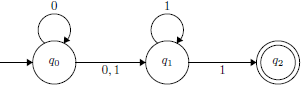
\includegraphics[width=\textwidth]{Problem 2 DFA}

\vspace{5mm}

\noindent\textbf{Solution:}

\vspace{5mm}

\newpage

\section*{Problem 3: [5 points]}

For any string $\omega$(over some alphabet $\sum$), let $\tilde{\omega}$ denote the reverse of $\omega$, i.e., writing $\omega$ from right to left. For example, if $\omega = bbbaba$ then $\tilde{\omega} = ababbb$. Furthermore, for any language $L$, let

\vspace{5mm}

$\tilde{L} = \{\tilde{\omega}|\omega \in L\},$

\vspace{5mm}

\noindent i.e., $\tilde{L}$ is the set of all strings that are the reverse of some string in $L$.

\vspace{5mm}

\noindent Prove that if $L$ is a regular language, then $\tilde{L}$ is also a regular language.

\vspace{5mm}

\noindent \textbf{Hint:} There might be multiple ways to prove this. I personally think the easiest way is to construct a regular expression that represents $\tilde{L}$.

\vspace{5mm}

\noindent\textbf{Solution:}

\end{document}